With the implementation and tests for the system presented, we can now conclude on the overall success of the project. To determine this, we first need to conclude whether or not the requirements, as described in section \ref{sec:moscow} and \ref{sec:non-requirements}, of the system has been fulfilled. From this it is assessed if the project overall works as an answer for the problem definition.

\section{Functional requirements}
Table \ref{conc:moscow} contains the current status of each requirement from the MoSCoW analysis. 

\begin{table}[H]
\centering
\begin{tabular}{|l|l|}
\hline
\textbf{Must have}                                                                                                                                                  & Fulfilled/Missing                 \\ \hline
\begin{tabular}[c]{@{}l@{}}Functionality to add and administrate citizens,\\ without need for a system administrator.\end{tabular}                                  & {\color[HTML]{e6e600} Partially-fulfilled} \\ \hline
\begin{tabular}[c]{@{}l@{}}Detect when a citizen has had a fall accident,\\ through input from the user on a device, such as a smartphone or wearable.\end{tabular} & {\color[HTML]{32CB00} Fulfilled} \\ \hline
Send an alarm to all of the citizen's contacts.                                                                                                                     & {\color[HTML]{32CB00} Fulfilled} \\ \hline
\textbf{Should have}                                                                                                                                                &                               \\ \hline
\begin{tabular}[c]{@{}l@{}}Detect when a citizen has had a fall accident, \\ through conversation with a personal assistant.\end{tabular}                           & {\color[HTML]{32CB00} Fulfilled} \\ \hline
\begin{tabular}[c]{@{}l@{}}Facilitate communication between a citizen and,\\ contact person during a fall accident.\end{tabular}                                    & {\color[HTML]{e6e600} Partially-fulfilled}                        \\ \hline
\textbf{Could have}                                                                                                                                                 &                               \\ \hline
\begin{tabular}[c]{@{}l@{}}Be able to integrate IoT devices and wearable tech.\end{tabular}                                        & {\color[HTML]{e6e600} Partially-fulfilled} \\ \hline
Associate device with a citizen to send alarms using device.                                                                                                        & {\color[HTML]{32CB00} Fulfilled} \\ \hline
Associate device with a contact person to receive alarms using device.                                                                                              & {\color[HTML]{32CB00} Fulfilled} \\ \hline
\textbf{Won't have}                                                                                                                                                 &                               \\ \hline
\begin{tabular}[c]{@{}l@{}}Automatically detect when a citizen has had a fall accident,\\ using a smartphone.\end{tabular}                                          & {\color[HTML]{CB0000} Missing} \\ \hline
\begin{tabular}[c]{@{}l@{}}Have a high accuracy when detecting a fall accident,\\ as defined in section \ref{sec:q-requirements}.\end{tabular}                    & {\color[HTML]{CB0000} Missing} \\ \hline
\end{tabular}
\caption{Pass/Fail of the project requirements}
\label{conc:moscow}
\end{table}

The table shows a status with one of three values: \textit{Fulfilled}, \textit{Partially-fulfilled} and \textit{Missing}, representing whether or not the required functionality to fulfill each requirement is present in the system. If a requirement is \textit{Fulfilled}, the functionality exist and is in a working state. \textit{Partially-fulfilled} can mean one of two things: the functionality exist but is not in a working state, or functionality for a subset of the requirement exists. Finally, if it is \textit{Missing}, the functionality is not available in the system, or in such a state that it does not work as intended.

\subsection{Missing functionality}
Two requirements are missing from the solution. These are:

\subsubsection{Automatically detect when a citizen has had a fall accident, using a smartphone.}\label{autofalldetect}
In the requirement specification, we decided not to include this requirement in the design and implementation of this project. This was due to the focus not being on app development during the project period.

\subsubsection{Have a high accuracy when detecting a fall accident, as defined in section \ref{sec:q-requirements}.}
Due to \ref{autofalldetect} not being implemented, this requirement is also missing from the final form of the project.

\subsection{Partially-fulfilled}
Three requirements are Partially fulfilled in system.

\subsubsection{Functionality to add and administrate citizens, without need for a system administrator.}
The functionality to fulfill this requirement exists, but is not implemented in the control panel. This is described in section \ref{sec:discussion:controlPanel}.


\subsubsection{Facilitate communication between citizen and contact person during a fall accident.}
This requirement is Partially fulfilled due to the fact that the app in certain situations performs a phone call instead of just sending notifications. It is however not possible to establish a two-way communication, without using phone calls, from the service. The system can however send out notifications to both citizens and contacts.


\subsubsection{Be able to integrate IoT devices.}
This requirement is Partially fulfilled as there technically is integration with IFTTT \ref{sec:iot}, but it has not been tested. This was mainly due to the lack of usable test devices.

\section{System criteria}
In this section, a conclusion on whether or not the system criteria presented in section \ref{sec:non-requirements} has been fulfilled is presented.

\subsection{Android app}
The android app works to a proof-of-concept degree. It can send out and receive alarms, and the relevant notifications for these. It can perform phonecalls, but cannot automatically detect a fall. 
\paragraph{Usability}
Since no usability test has been made on the App, it is hard to evaluate its usability. As such, this criteria is not currently fulfilled.

\paragraph{Efficient}
To perform a basic test, we used a Samsung Galaxy S5. This smartphone can show app energy use down to 0.01\% of usage per hour.

\begin{figure}[h]
    \centering
    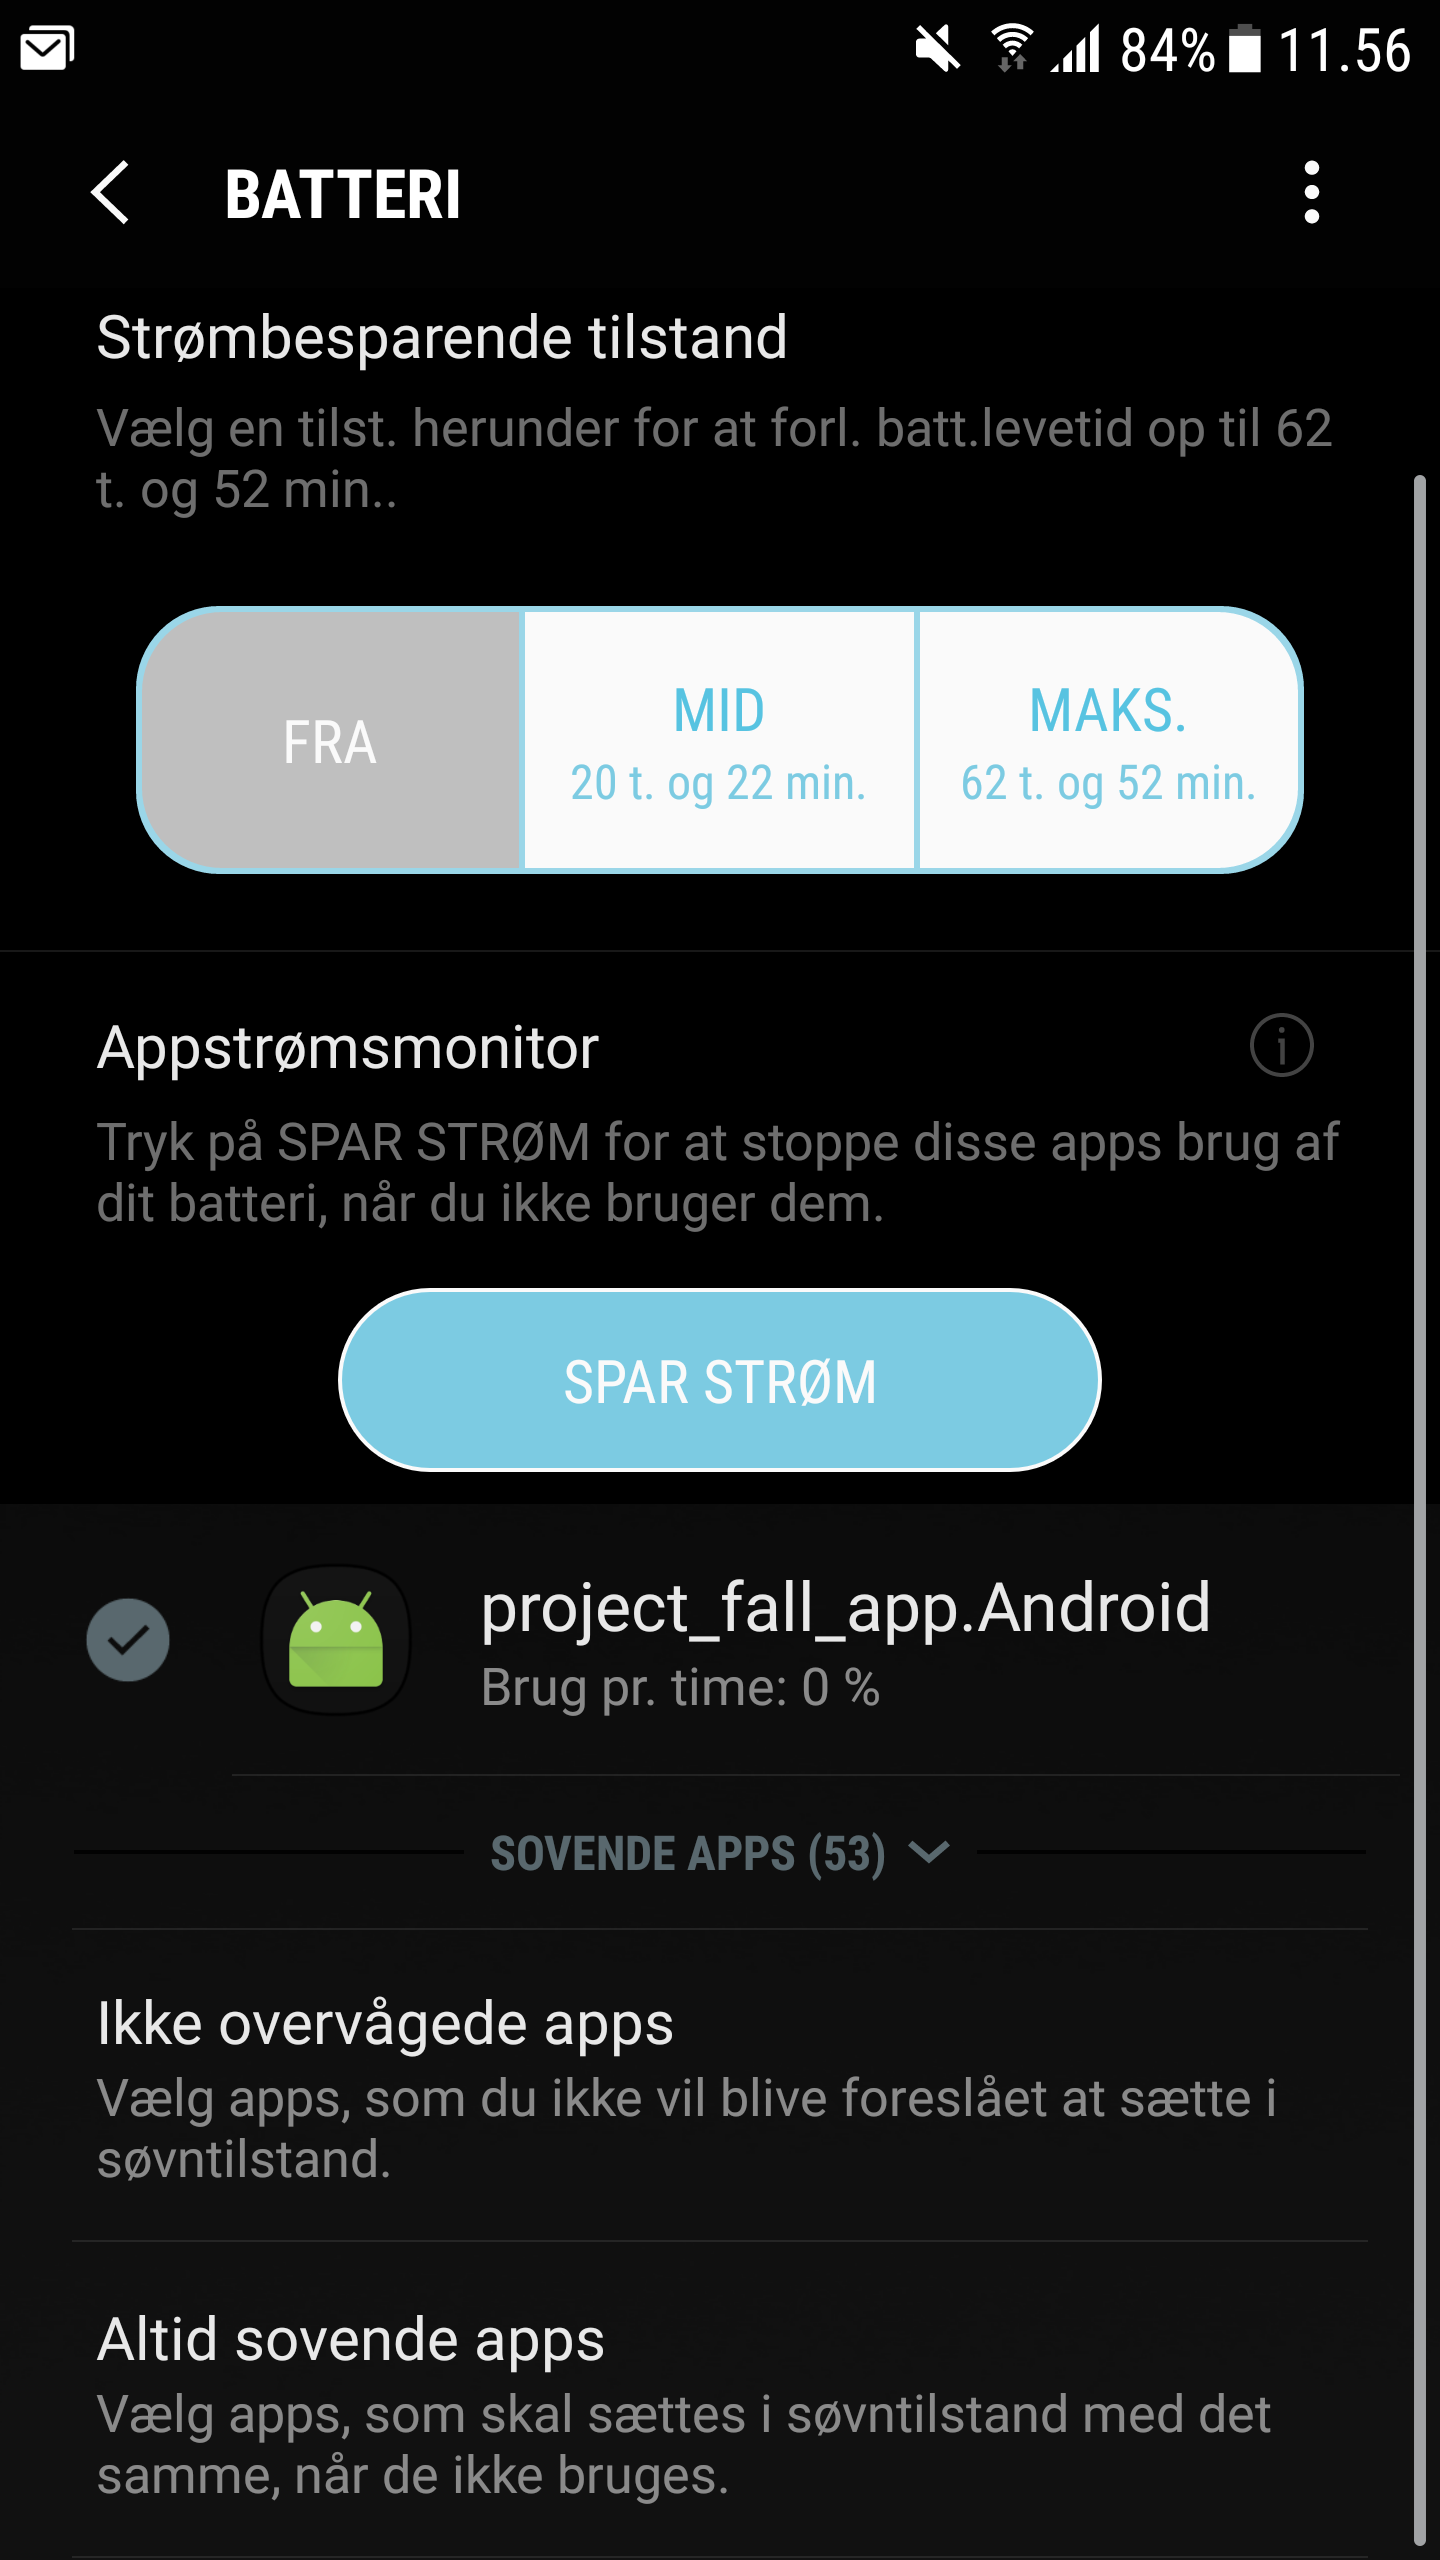
\includegraphics[scale=0.1]{Figures/batteryUsiged.png}
    \caption{Battery used in hour}
    \label{fig:batteryUsed}
\end{figure}

After running the app for a few hours, it still showed 0.00\% on the battery usage statistics. This is shown on \ref{fig:batteryUsed}.
So, using this statistic, it can be concluded that the app is efficient enough that it will not impact battery life significantly.

\paragraph{Correct}
Considering the requirements from the MoSCoW analysis, without the requirements that was defined as \textit{won't have}, the App can be considered correct. 

\paragraph{Reliable}
Disregarding fall detection, which it was decided not to implement, the app can be considered reliable, since it delivers the correct notifications and alarms.

\paragraph{Testable}
The App is highly testable, since the development environment and framework makes it possible to write unit-tests for the different parts of the app. 

\paragraph{Portable}
The App can be considered portable, since it is written in a cross platform environment, as described in section \ref{sec:crossplat}.


\subsection{Personal assistant}
The personal assistant was in a working state when the project reached its final form.
\paragraph{Usability}
As with the previous case, no usability test has been made on the personal assistant, and as such an evaluation of the usability of the personal assistant cannot be performed.

\paragraph{Correct}
The personal assistant fulfills the requirements outlined in the MoSCoW analysis except for the fact that a special keyword has to be used when interacting with the assistant. This was a limitation encountered in the personal assistant's software.

\paragraph{Reliable}
During the development process, it was discovered that the voice detection service was not very reliable in how well it picked up verbal commands. Due to this, the personal assistant cannot be considered reliable.

\paragraph{Testable}
While the personal assistant was not tested directly, its functionality was tested through the integration test performed in \ref{sec:integration-test}.



\subsection{Web-service}
As with the personal assistant, the web-service was in a working proof-of-concept state when the project reached its final form.
\paragraph{Secure}
Due to the fact that the web-service utilizes HTTPS and authorization through the usage of IAM resources (IAM Policies, \ref{sec:iam}), it can be considered secure, unless Amazon's own services are somehow insecure.

\paragraph{Efficient}
No specific testing was performed on the efficiency of the web-service, but it is assumed that Amazons services are relatively performant.%its a word i looked it up

\paragraph{Correct}
The web-service is correct in most aspects, except for the cases where it provides all users to a citizen admin instead of just the ones administrated by that admin. 

\paragraph{Reliable}
The web-service is reliable, in the cases that we actually fulfill. The only case where it is not reliable, is as mentioned in the previous paragraph, when providing citizens to a citizen admin.

\paragraph{Maintainable}
The web-service is maintainable, as it is separated into relatively small code files (consisting of Lambda functions, which is then uploaded to the AWS service).

\paragraph{Testable}
The web-service is easily testable, due to it consisting of relatively small code parts (A lambda function per file), and due to having full access to all the endpoints from where ever the test is to be performed.

\paragraph{Flexible}
All parts of the web-service is centralized, the internal architecture is well structured and the functionality related to the different endpoints of the API is well separated. This results in low costs related to potential changes to the service, as long as no changes is made to the structure of the API, since this would require changes to all components that makes use of these.

\paragraph{Interoperable}
The web-service is easily interoperable, as it allows for coupling with smartphones directly and other devices through IFTTT.

\subsection{Control panel}
The control panel was in a working state at the projects conclusion, although it was missing some functionality. 
\paragraph{Usability}
As with the app and the personal assistant, no usability testing has been performed, and again, no evaluation can be made of this criteria.

\paragraph{Secure}
The control panel is secure, from a technical standpoint. This is much the same as why the web-service is secure, due to https and authentication.

\paragraph{Correct}
The control panel is mostly correct, but missing some functionality due to lacking backend functionality. There is also a few functions missing in the control-panel due to time constraints. This is described in section \ref{sec:discussion:controlPanel}.

\section{Problem definition}
With the different requirements and criteria for the system evaluated, we can now conclude on the overall success of the project, by evaluating whether or not we have succeeded to answer the problem definition:

\begin{figure}[H]
    \begin{center}
        \textit{How can the problem of fall accidents, where the citizen is not able to get up by themselves, be assisted by a smart solution, integrating smartphones and personal assistant technologies in a web based solution?}
    \end{center}
\end{figure}

Since no test has been made on any actual users, it is hard to evaluate whether or not the system has, if implemented, any positive impact on citizens in risk of having a fall accident. Considering the design, found in part \ref{chap:design}, and the results from the previous sections of this chapter, we believe that the system and project described throughout this report fits as an answer for the problem definition. That said, the system is currently only at a proof-of-concept state. What is needed to go from this state to a finished product, that can actually be deployed to the target audience, is described in chapter \ref{chap:future-work}. Since our system integrates both IoT, a smart assistant, a smartphone, does not need any significant technical setup to work and performs its services automatically, we believe that it can be considered to be a smart solution to the problem.